\documentclass[12pt,a4paper]{article}
\usepackage[utf8]{inputenc}
\usepackage[T1]{fontenc}
\setcounter{secnumdepth}{5}
\usepackage[francais, english]{babel}
\AddThinSpaceBeforeFootnotes % notes de bas de page
\FrenchFootnotes % notes de bas de page
\usepackage{lmodern}		%Pour changer le pack de police
\usepackage[pdftex]{graphicx}% Pour inclure les images
\usepackage{gensymb}\usepackage{pdfpages}
\usepackage[numbers]{natbib}
\usepackage{amsmath}
\usepackage{caption}
\usepackage{float}
\usepackage{fullpage}
\usepackage{amssymb}
\usepackage{mathrsfs}
\usepackage{textcomp}
\usepackage{enumitem}
\frenchbsetup{StandardLists=True}%pour les listes 
\usepackage{array}	%To build arrays
\usepackage[version=3]{mhchem}
\usepackage{colortbl}
\usepackage{textcomp}%euros
\usepackage{hyperref}
\usepackage{color}
\usepackage{url}
\usepackage{comment} %pour faire des coms
\usepackage{transparent}
\usepackage{eso-pic}
\usepackage{setspace}
\makeatletter
\renewcommand\theequation{\thesection.\arabic{equation}}
\@addtoreset{equation}{section}
\makeatother
\usepackage{verbatim}
\usepackage{setspace}
\onehalfspacing
\usepackage{etex}
\usepackage{m-pictex,m-ch-en}

%\usepackage{fullpage}
\usepackage{geometry}
\geometry{top=2.5cm,bottom=2.6cm,left=2.7cm,right=2.5cm}
%\begin{document}
\newcommand\HRule{\rule{\textwidth}{1pt}}

%pour l'image :


% 1 : Logo ulb en fond
\newcommand\BackgroundPic{%
    \put(0,0){%
        \parbox[b][\paperheight]{\paperwidth}{%
            \vfill
            \centering
            {\transparent{0.07}
\includegraphics[width=1\textwidth]{Scientiae.jpg}}%
            \vfill
        }
    }
}
% 2 : banderolle ulb en dessous 
\newcommand\BackgroundPicE{%
    \put(0,0){%
        \parbox[c][\paperheight]{\paperwidth}{%
            \vfill
            \centering
            {\transparent{1}
\includegraphics[width=1.25\textwidth]{ulb.png}}%
            \vfill
        }
    }
}


%%%%%%%%%%%%%%%%%%%%%%%%%%%%%%%%%%%%%%%%%%

%%%%%%%%%%%%%%%%%%%%%%%%%%%%%%%%%%%%%%%%%%%%%%%%%%%%%%%%%%%
\begin{document}
%-----------------------PREMIERE PAGE-----------
\AddToShipoutPicture*{\BackgroundPic}
\AddToShipoutPicture*{\BackgroundPicE}

\begin{titlepage}

\begin{center}

% Upper part of the page
%\textsc{\LARGE Brussels Faculty of Engineering}\\[1.2cm]


\includegraphics[width=1\textwidth]{Logos.pdf}\\[1.2cm]

\textsc{\Large Master of science in chemical engineering}\\[3cm]

% Title
\HRule \\[0.4cm]
{ \huge \bfseries Mechanics of materials: laboratories}\\[0.4cm]

\HRule \\[0.5cm]%[4cm]

%\begin{figure}[!h]
    %%\centering
    %\includegraphics[width=0.4\textwidth]{CPYOURI.jpeg}
    %\caption{Conductimètre employé}
%\end{figure} 




\begin{minipage}{0.45\textwidth}
\begin{flushleft} \large
\begin{doublespace}
\emph{Author : }\\
\end{doublespace}
%Nos Noms alignés par ordre alphab
\begin{tabular}{ll}
Léonard G.&\textbf{Darago}\\
Thomas B.&\textbf{Gillet}\\


\end{tabular}
%%%%%%%%%%%
\end{flushleft}
\end{minipage}
\begin{minipage}{0.45\textwidth}
\begin{flushleft} \large
\begin{doublespace}
\emph{Teacher : }\\ %% /!\ penser à mettre au pluriel si nécessaire
\end{doublespace}
%Nos Noms alignés par ordre alphab
\begin{tabular}{ll} 
Thierry J. &\textbf{Massart}\\



\end{tabular}
%%%%%%%%%%%
\end{flushleft}
\end{minipage}

\vfill

% Bottom of the page
%\includegraphics[width=0.5\textwidth]{LogoEPB.jpg}\\[0.4cm]
\selectlanguage{english}
{\large Academic year 2017-2018}\\


\end{center}

\end{titlepage} 
\section*{Running a linear analysis}
\subsection*{Question 1}
There are three elements in a node, three nodes per triangle; this means that there are 2 nodes per side of the triangle,the interpolation is therefore linear. Since the displacement field is linear and the solution is searched using linear functions, the exact solution will be found numerically. The problem is linear. since in the final element approximation there is a connection between the number of nodes and the degree of the form functions that are used. 

\begin{figure}[h!]
\centering
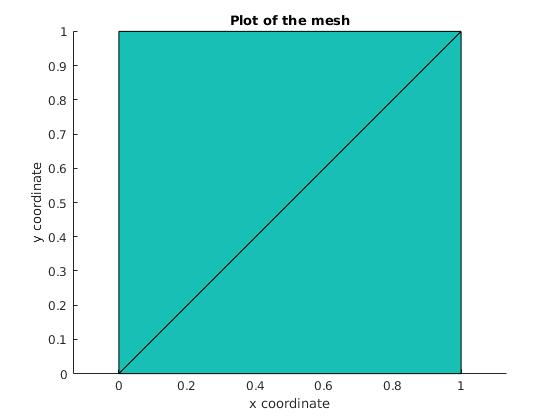
\includegraphics[width=10cm]{ex1_mesh.jpg}
\caption{Mesh of the first exercise with a node at each corner.}
\end{figure}

\subsection*{Question 2}
It is not because there is no load in the data files that there is no loading, it can hence be applied through imposed displacement. 
\subsection*{Question 3}
When the computation is run there are different steps. At each step, it is supposed that the structure behaves linearly. If the problem is not linear and we suppose that we are in a linear case, then at each step it would have been necessary to realize several iteration. Since only one iteration is necessary at each step, it means that the problem is linear.
\subsection*{Question 4}


\section*{Running a geometrically non-linear analysis}
\subsection*{Question 5}
At a first glimpse, the two files \verb|square_compress.m and square_compress_lin.m| look similar.
The main difference is that the outputs of those two files are different. 
\\On a first hand,in \verb|square_compress_lin.m| the output are :
\begin{itemize}
\item The displacement
\item The strain
\item The stress
\end{itemize}
All those outputs are linear.
\\On the second hand, \verb|square_compress.m| has non-linear outputs:
\begin{itemize}
\item The displacement
\item pkstrs
\item Green deformation
\end{itemize}
The non-linearity of the \verb|square_compress.m| outputs is the presence of the Green deformation.
$\epsilon_{Green}=\frac{1}{2}(\lambda^2 -1)$.
The maximal iteration authorized are set to 7 for the linear file and to 20 for the non-linear file. However, when the code is executed, the results are obtained in 1 iteration for the compress.m and in 2 iterations for the \verb|square_compress.m|There is only two iteration needed for the non-linear file since one stopped when the difference between the applied load and the load one want is below the tolerance that is set at $10^{-7}$ in the code.
\\
\\The Poisson coefficient is high for rubbery-like materials since for this kind of materials there is no change of volume, it is incompressible.
\\
\\The law as the same form, but relates to quantities that are different, it is an hyperelastic law.
\\
\\Validity domain, was defined by ourself at 1\%. Works until the $11^{th}$ iteration and thus till a force of $1\times 10^{-1}$

\section*{Effect of a rigid body rotation on the simulation results}
\subsection*{Question 6}


$\{F_i\}=\int_{V} (B_{(q)})^t\{S_{(q)}\}dV$
but $\{B_{(q)}\}$ and $\{S_{(q)}\}$ are defined differently in the two cases.
The evanouissantes deformation tensor is not objective, while the Green tensor is.
\\The modelling assumptions that has to be taken in order to have the same response given by those two elements is to say we have small angles.



\section*{Plasticity around a hole}
\subsection*{Question 7}
Les contraintes ne dépendent que de la déformation élastique. Deformation élastique= déformation totale-déformation plastique.

If we plots the les contraintes in elastic cases, it will not change anything. The only change will be the signification of the colour, but la carte de la répartitions des couleurs sera la même.
\\In the plastic case, la carte des contraintes va changer au cours du chargement.
Comme il n'y a pas de distribution uniforme des contraintes spatiales, on a une redistribution de contraintes. La contraintes ne se distribue alors pas de manière uniforme dans le matériau. certains endroits vont alors rentrer en plasticité plus vite --> la réaction instantannée du matériau devient alors beaucoup plus douce.

\section*{Detecting the onset of necking in a tensile test
}

\subsection*{Question 8}

\section*{
Simulation of an extrusion process}
\subsection*{Question 9}
\end{document}


